% !TEX root =  master.tex
\cleardoublepage
\section{Methoden für PCR-Pooling}
In diesem Kapitel sollten Methoden für das PCR-Pooling beschrieben werden.
Begonnen wird mit einem einfachen, eindimensionalen Poolingverfahren als spätere Referenz.
Kompliziertere Verfahren werden später erläutert und gegenübergestellt.
Hierdurch wird sichergestellt, dass das einfachstmögliche Verfahren angewandt wird.
Umfangreiche Methoden werden nur weiter verfolgt, wenn sie das einfache Referenzverfahren übertreffen.

\subsubsection{Minipool}
Das einfachste Verfahren für Pooling ist, eine eindimensionale Reihe von Proben zu verwenden und diese vor der PCR-Analyse zu kombinieren.
Die Matrix lässt sich hierbei als 1xN beschreiben.
Die Proben werden gemeinsam getestet.
\begin{itemize}
	\item \textbf{Negatives Poolergebnis:}\newline
	Ein negatives Gesamtergebnis bedeutet, dass \textbf{jede Einzelprobe negativ} war.
	
	Es wurde somit durch einen Test festgestellt, dass alle Personen im Pool negativ sind.
	
	Die Effizienz lässt sich somit beschreiben als $\frac{Anzahl Testpersonen (N)}{Anzahl Tests (1)} $.
	
	\item \textbf{Positives Poolergebnis:}\newline
	Ein positives Gesamtergebnis bedeutet, dass \textbf{mindestens eine Einzelprobe positiv} war.
	
	In diesem Fall müssen weitere Tests durcheführt werden, um die positiven Einzelpersonen zu ermitteln.
	Die Tests erfolgen hierbei nacheinander und sind statistisch unabhängig voneinander.
	
	Die Nachtestung kann durch mehrstufiges Pooling optimiert werden.
	Für das einfachste Basisverfahren wird allerdings angenommen, dass nach einem Positivergebnis das Pooling beendet wird.
	Die Personen innerhalb des positiven Pools werden einzeln nachgetestet.
	
	Im Falle einer Nachtestung wird somit ein initialer Test für den Pool benötigt, welcher positiv ausfällt.
	Danach werden nochmal Tests für jede Einzelperson benötigt.
	
	Die Effizienz lässt sich somit beschreiben als $\frac{Anzahl Testpersonen (N)}{1 Pooltest + N Einzeltests} $.
\end{itemize}


Die Testung erfolgt zweistufig.

Der Erwartungswert für die benötigte Anzahl der Tests lässt sich beschreiben als:

Wenn(Pool Positiv)
Dann -> N+1
Andernfalls -> 1

Der erwartete Testbedarf hängt ab von der Wahrscheinlichkeit, dass der Pool positiv ist.
Dieser lässt sich durch die prozentuale Angabe der Testprävalent ermitteln.

% \cleardoublepage
\subsubsection{Effizienzkurve Minipool}
Hieraus ergibt sich:
%Erwartungswert Testbedarf = (P(Positiv) * N+1) + (!P(Positiv) * 1)
%N/((MIN(1;N*Prävalenz)*(N+1))+(1-MIN(1;N*Prävalenz)))

P(PoolPositiv) = $(min\left(1;Poolsize\cdot Pravalenz\right)$

Erwartungswert Personen pro Test =
$\frac{Poolsize}{P(PoolPositiv)\cdot (Poolsize + 1)) + (1 - P(PoolPositiv))}$

\begin{figure}[h]
	\centering
	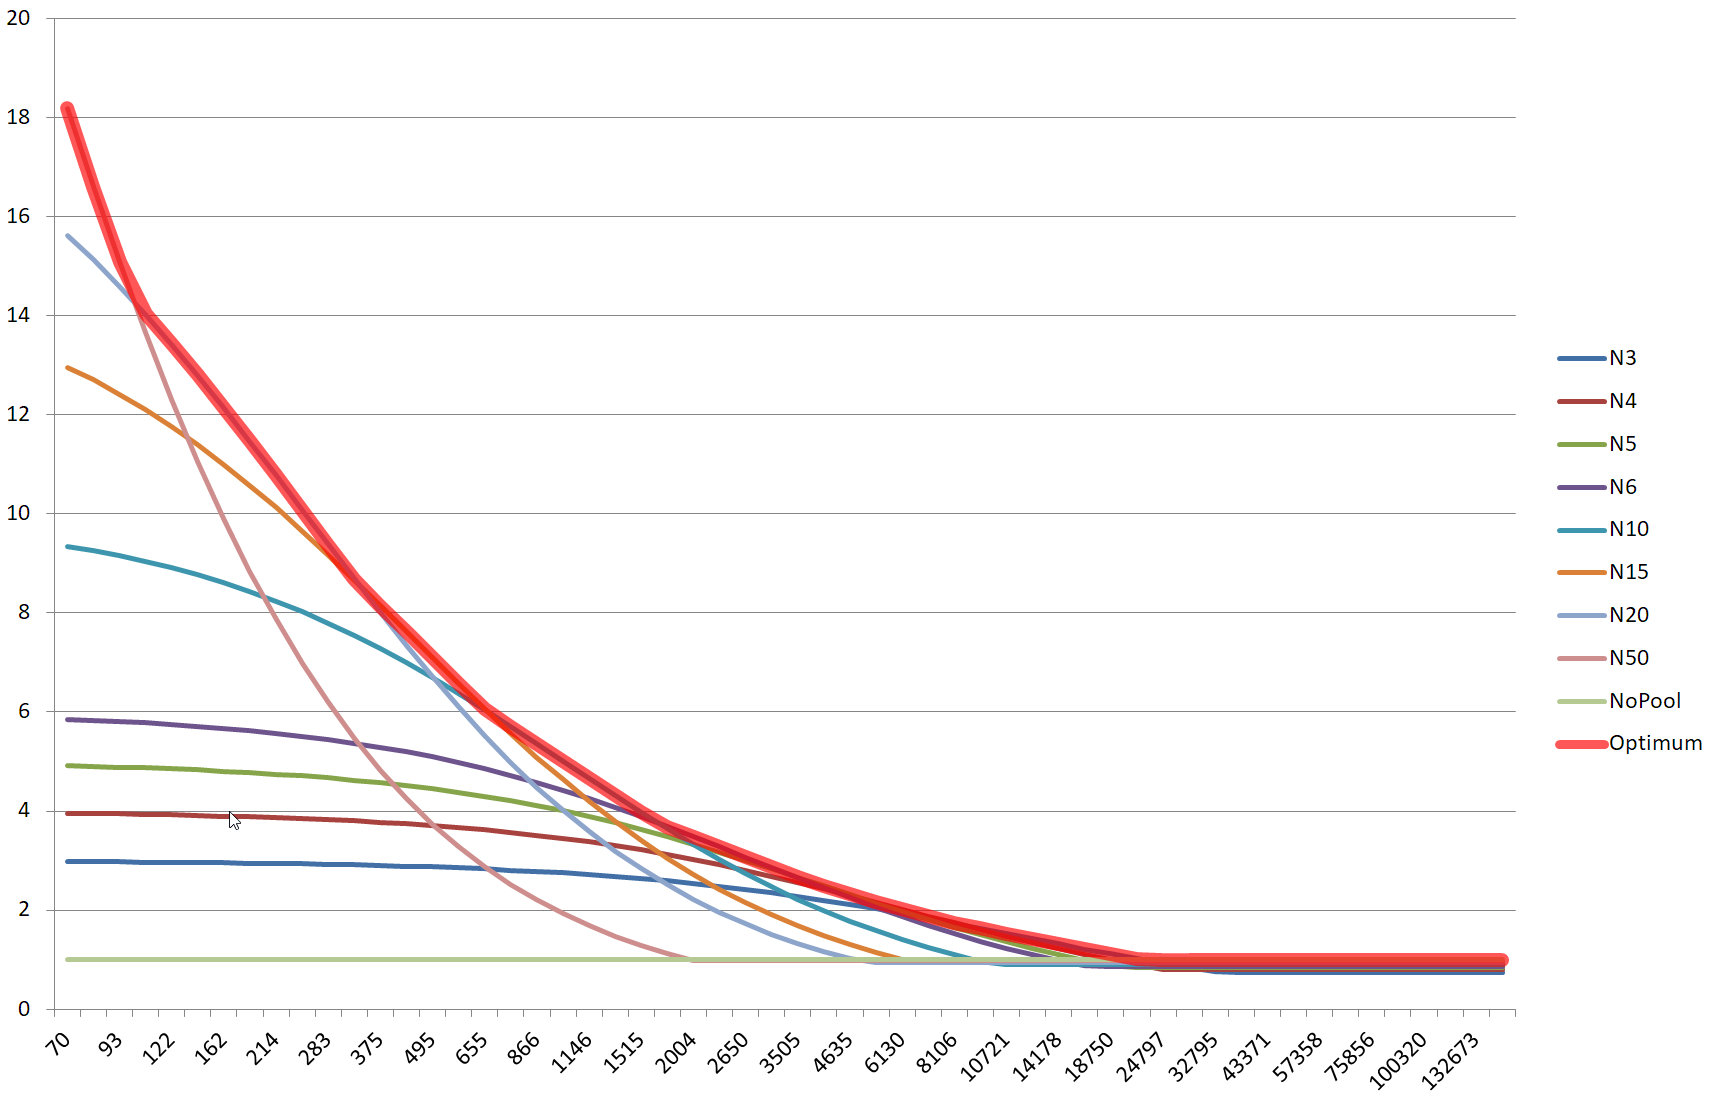
\includegraphics[height=.6\textwidth]{img/Minipool}
	%\caption{Geplanter Aufbau der Arbeit\footnotemark}
\end{figure}

\cleardoublepage
